\documentclass[border=6pt]{standalone}
\usepackage{tikz}
\usetikzlibrary{arrows.meta,positioning,shapes.geometric}
\begin{document}
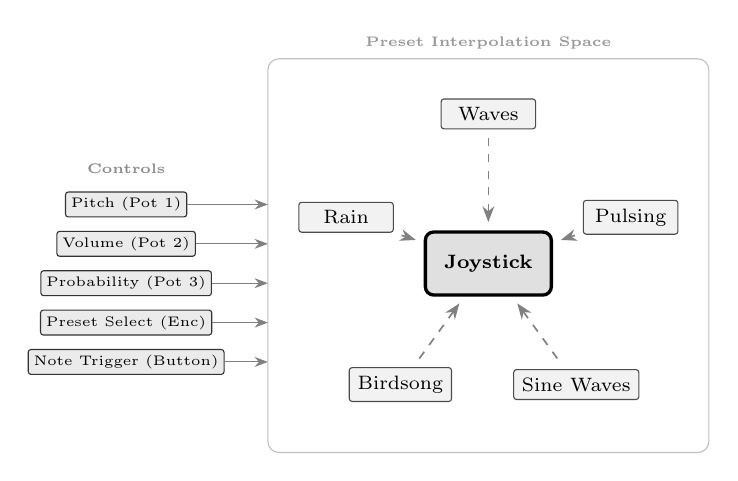
\begin{tikzpicture}

\node[rectangle, draw=black, very thick, fill=black!12, rounded corners=3pt, font=\scriptsize\bfseries, inner sep=4pt, minimum height=0.8cm, minimum width=1.6cm] (joy) at (0, 0) {Joystick};

\node[rectangle, draw=black!70, fill=black!5, rounded corners=1pt, font=\scriptsize, inner sep=3pt, minimum width=1.2cm, align=center] (p1) at (90:1.9cm) {Waves};
\node[rectangle, draw=black!70, fill=black!5, rounded corners=1pt, font=\scriptsize, inner sep=3pt, minimum width=1.2cm, align=center] (p2) at (162:1.9cm) {Rain};
\node[rectangle, draw=black!70, fill=black!5, rounded corners=1pt, font=\scriptsize, inner sep=3pt, minimum width=1.2cm, align=center] (p3) at (234:1.9cm) {Birdsong};
\node[rectangle, draw=black!70, fill=black!5, rounded corners=1pt, font=\scriptsize, inner sep=3pt, minimum width=1.2cm, align=center] (p4) at (306:1.9cm) {Sine Waves};
\node[rectangle, draw=black!70, fill=black!5, rounded corners=1pt, font=\scriptsize, inner sep=3pt, minimum width=1.2cm, align=center] (p5) at (18:1.9cm) {Pulsing};

\draw[Stealth-, dashed, black!50, semithick, shorten <=3pt, shorten >=3pt] (joy) -- (p1);
\draw[Stealth-, dashed, black!50, semithick, shorten <=3pt, shorten >=3pt] (joy) -- (p2);
\draw[Stealth-, dashed, black!50, semithick, shorten <=3pt, shorten >=3pt] (joy) -- (p3);
\draw[Stealth-, dashed, black!50, semithick, shorten <=3pt, shorten >=3pt] (joy) -- (p4);
\draw[Stealth-, dashed, black!50, semithick, shorten <=3pt, shorten >=3pt] (joy) -- (p5);

\draw[black!25, rounded corners=4pt] (-2.8, 2.6) rectangle (2.8, -2.4);
\node[font=\tiny\bfseries, text=black!40] at (0, 2.8) {Preset Interpolation Space};

\node[rectangle, draw=black!80, fill=black!8, rounded corners=1pt, font=\tiny, inner sep=2pt] (c1) at (-4.6, 0.75) {Pitch (Pot 1)};
\node[rectangle, draw=black!80, fill=black!8, rounded corners=1pt, font=\tiny, inner sep=2pt] (c2) at (-4.6, 0.25) {Volume (Pot 2)};
\node[rectangle, draw=black!80, fill=black!8, rounded corners=1pt, font=\tiny, inner sep=2pt] (c3) at (-4.6, -0.25) {Probability (Pot 3)};
\node[rectangle, draw=black!80, fill=black!8, rounded corners=1pt, font=\tiny, inner sep=2pt] (c4) at (-4.6, -0.75) {Preset Select (Enc)};
\node[rectangle, draw=black!80, fill=black!8, rounded corners=1pt, font=\tiny, inner sep=2pt] (c5) at (-4.6, -1.25) {Note Trigger (Button)};

\draw[-Stealth, thin, black!50] (c1.east) -- (-2.8, 0.75);
\draw[-Stealth, thin, black!50] (c2.east) -- (-2.8, 0.25);
\draw[-Stealth, thin, black!50] (c3.east) -- (-2.8, -0.25);
\draw[-Stealth, thin, black!50] (c4.east) -- (-2.8, -0.75);
\draw[-Stealth, thin, black!50] (c5.east) -- (-2.8, -1.25);

\node[font=\tiny\bfseries, text=black!45] at (-4.6, 1.2) {Controls};

\end{tikzpicture}
\end{document}
